\begin{knitrout}
\definecolor{shadecolor}{rgb}{1, 1, 1}\color{fgcolor}\begin{kframe}
\begin{alltt}
\hlstd{dens.np.df} \hlkwb{<-} \hlkwd{data.frame}\hlstd{(}\hlkwc{x} \hlstd{= dens.np}\hlopt{$}\hlstd{eval[,} \hlnum{1}\hlstd{],} \hlkwc{y} \hlstd{= dens.np}\hlopt{$}\hlstd{dens)}

\hlkwd{ggplot}\hlstd{(x_df,} \hlkwd{aes}\hlstd{(x))} \hlopt{+}
 \hlkwd{geom_histogram}\hlstd{(}
   \hlkwd{aes}\hlstd{(}\hlkwc{y} \hlstd{= ..density..),}
   \hlkwc{binwidth} \hlstd{= h_cv_np_ml}\hlopt{$}\hlstd{bw,}
   \hlkwc{col} \hlstd{=} \hlstr{"black"}\hlstd{,}
   \hlkwc{fill} \hlstd{=} \hlstr{"white"}
 \hlstd{)} \hlopt{+}
 \hlkwd{stat_function}\hlstd{(}
   \hlkwc{fun} \hlstd{= dnorm,}
   \hlkwc{args} \hlstd{=} \hlkwd{list}\hlstd{(}\hlkwc{mean} \hlstd{= mu,} \hlkwc{sd} \hlstd{= sigma),}
   \hlkwc{color} \hlstd{=} \hlstr{"red"}
 \hlstd{)} \hlopt{+}
 \hlkwd{geom_line}\hlstd{(}\hlkwc{data} \hlstd{= dens.np.df,} \hlkwd{aes}\hlstd{(x, y),} \hlkwc{color} \hlstd{=} \hlstr{"blue"}\hlstd{)} \hlopt{+}
 \hlkwd{theme_minimal}\hlstd{(}\hlkwc{base_size} \hlstd{=} \hlnum{20}\hlstd{)}
\end{alltt}
\end{kframe}
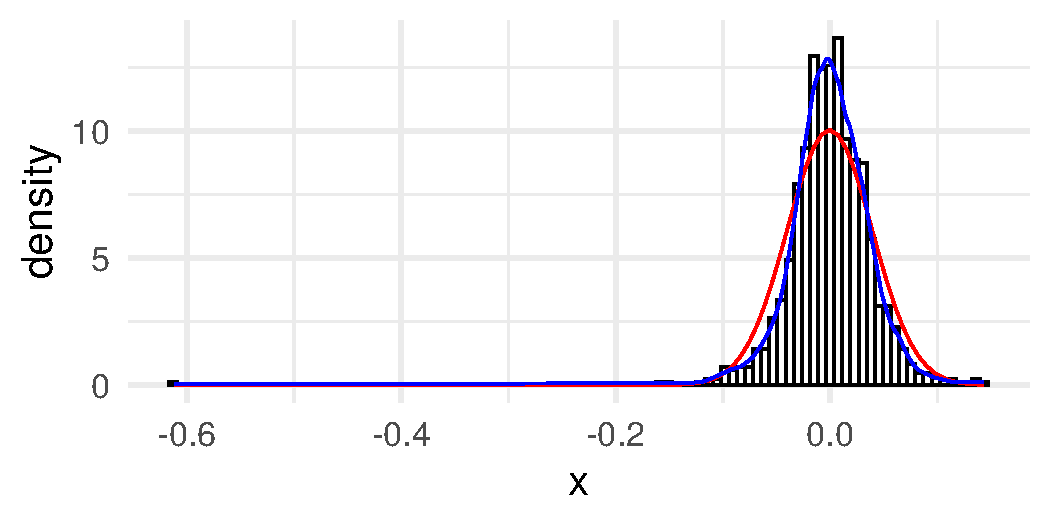
\includegraphics[width=\maxwidth]{figure/unnamed-chunk-31-1} 

\end{knitrout}
